\chapter{概率}

\index{probability}

\key{概率}是 0 到 1 之间的实数，用来表示一个事件发生的可能性。必然事件的概率为 1，不可能事件的概率为 0。事件的概率记作 $P(\cdots)$，括号中的省略号描述该事件。

例如，掷一枚骰子的结果是 1 到 6 之间的整数，每种结果的概率均为 $1/6$。可以得到以下概率：

\begin{itemize}[noitemsep]
\item $P(\textrm{“结果为 4”})=1/6$
\item $P(\textrm{“结果不是 6”})=5/6$
\item $P(\textrm{“结果为偶数”})=1/2$
\end{itemize}

\section{概率计算}

计算事件概率时，可以使用组合数学，也可以模拟生成事件的过程。例如，计算从洗好的牌中抽出三张点数相同的牌的概率（如 $\spadesuit 8$、$\clubsuit 8$、$\diamondsuit 8$）。

\subsubsection*{方法一}

可以使用公式

\[\frac{\textrm{目标结果数}}{\textrm{全部结果数}}.\]

本题的目标结果是三张牌点数相同。这样的结果共有 $13 {4 \choose 3}$ 种，因为点数有 13 种选择，从 4 种花色中选择 3 种有 ${4 \choose 3}$ 种方法。

全部结果共有 ${52 \choose 3}$ 种，因为要从 52 张牌中选择 3 张。因此，事件概率为

\[\frac{13 {4 \choose 3}}{{52 \choose 3}} = \frac{1}{425}.\]

\subsubsection*{方法二}

另一种计算方法是模拟生成事件的过程。本例抽取三张牌，因此过程分为三步，并要求每一步都成功。

抽取第一张牌必然成功，因为没有任何限制。第二步成功的概率为 $3/51$，因为剩余 51 张牌中有 3 张与第一张点数相同。类似地，第三步成功的概率为 $2/50$。

整个过程成功的概率为

\[1 \cdot \frac{3}{51} \cdot \frac{2}{50} = \frac{1}{425}.\]

\section{事件}

概率论中的事件可以表示为集合
\[A \subset X,\]
其中 $X$ 包含所有可能结果，$A$ 是其中一部分结果。例如，掷骰子的结果集合为
\[X = \{1,2,3,4,5,6\}.\]
事件“结果为偶数”对应集合
\[A = \{2,4,6\}.\]

为每个结果 $x$ 赋予概率 $p(x)$，则事件 $A$ 的概率 $P(A)$ 可按公式
\[P(A) = \sum_{x \in A} p(x).\]
求得，即对事件中各结果的概率求和。例如，掷骰子时，每个结果 $x$ 都有 $p(x)=1/6$，所以事件“结果为偶数”的概率为
\[p(2)+p(4)+p(6)=1/2.\]

结果集合 $X$ 中各结果的总概率必须为 1，即 $P(X)=1$。

由于概率论中的事件是集合，可以使用标准集合运算处理它们：

\begin{itemize}
\item \key{补集} $\bar A$ 表示“$A$ 不发生”。例如，掷骰子时，$A=\{2,4,6\}$ 的补集为 $\bar A = \{1,3,5\}$。
\item \key{并集} $A \cup B$ 表示“$A$ 或 $B$ 发生”。例如，$A=\{2,5\}$ 与 $B=\{4,5,6\}$ 的并集为 $A \cup B = \{2,4,5,6\}$。
\item \key{交集} $A \cap B$ 表示“$A$ 和 $B$ 同时发生”。例如，$A=\{2,5\}$ 与 $B=\{4,5,6\}$ 的交集为 $A \cap B = \{5\}$。
\end{itemize}

\subsubsection{补集}

补集 $\bar A$ 的概率按公式
\[P(\bar A)=1-P(A).\]

计算。有时可以通过求相反事件，利用补集轻松解决问题。例如，掷骰子十次至少出现一次 6 的概率为
\[1-(5/6)^{10}.\]

其中 $5/6$ 是单次结果不为 6 的概率，$(5/6)^{10}$ 是十次结果均不为 6 的概率；它的补集就是答案。

\subsubsection{并集}

并集 $A \cup B$ 的概率按公式
\[P(A \cup B)=P(A)+P(B)-P(A \cap B).\]
计算。例如，掷骰子时，事件
\[A=\textrm{“结果为偶数”}\]
与
\[B=\textrm{“结果小于 4”}\]
的并集为
\[A \cup B=\textrm{“结果为偶数或小于 4”},\]
其概率为
\[P(A \cup B) = P(A)+P(B)-P(A \cap B)=1/2+1/2-1/6=5/6.\]

如果事件 $A$、$B$ \key{互斥}，即 $A \cap B$ 为空，则

\[P(A \cup B)=P(A)+P(B).\]

\subsubsection{条件概率}

\index{conditional probability}

\key{条件概率}
\[P(A | B) = \frac{P(A \cap B)}{P(B)}\]
表示在 $B$ 发生的条件下 $A$ 的概率。因此，计算 $A$ 的概率时，只考虑同时属于 $B$ 的结果。

对于前面的集合，
\[P(A | B)= 1/3,\]
因为 $B$ 的结果为 $\{1,2,3\}$，其中一个是偶数。这就是已知结果位于 $1 \ldots 3$ 时，结果为偶数的概率。

\subsubsection{交集}

\index{independence}

利用条件概率，交集 $A \cap B$ 的概率可按公式
\[P(A \cap B)=P(A)P(B|A).\]
计算。如果
\[P(A|B)=P(A) \hspace{10pt}\textrm{且}\hspace{10pt} P(B|A)=P(B),\]
则称事件 $A$、$B$ \key{相互独立}，即 $B$ 是否发生不改变 $A$ 的概率，反之亦然。此时交集的概率为
\[P(A \cap B)=P(A)P(B).\]
例如，从一副牌中抽牌时，事件
\[A = \textrm{“花色为梅花”}\]
与
\[B = \textrm{“点数为 4”}\]
相互独立。因此，事件
\[A \cap B = \textrm{“抽到梅花 4”}\]
的概率为
\[P(A \cap B)=P(A)P(B)=1/4 \cdot 1/13 = 1/52.\]

\section{随机变量}

\index{random variable}

\key{随机变量}是由随机过程产生的数值。例如，掷两枚骰子时，可以定义随机变量
\[X=\textrm{“两次结果之和”}.\]
如果结果为 $[4,6]$（即先掷出 4，再掷出 6），则 $X$ 的值为 10。

用 $P(X=x)$ 表示随机变量 $X$ 取值为 $x$ 的概率。例如，掷两枚骰子时，$P(X=10)=3/36$，因为全部结果有 36 种，而得到和 10 的方式有三种：$[4,6]$、$[5,5]$、$[6,4]$。

\subsubsection{期望值}

\index{expected value}

\key{期望值} $E[X]$ 表示随机变量 $X$ 的平均值，可计算为
\[\sum_x P(X=x)x,\]
其中 $x$ 遍历 $X$ 的所有可能取值。

例如，掷一枚骰子的期望结果为
\[1/6 \cdot 1 + 1/6 \cdot 2 + 1/6 \cdot 3 + 1/6 \cdot 4 + 1/6 \cdot 5 + 1/6 \cdot 6 = 7/2.\]

期望值的一个重要性质是\key{线性性}：$E[X_1+X_2+\cdots+X_n]$ 始终等于 $E[X_1]+E[X_2]+\cdots+E[X_n]$。即使这些随机变量相互依赖，公式仍然成立。

例如，掷两枚骰子时，点数和的期望为
\[E[X_1+X_2]=E[X_1]+E[X_2]=7/2+7/2=7.\]

考虑把 $n$ 个球随机放入 $n$ 个盒子，并计算空盒子数量的期望。每个球等概率地放入任意盒子。例如，当 $n=2$ 时，所有可能情况如下：
\begin{center}
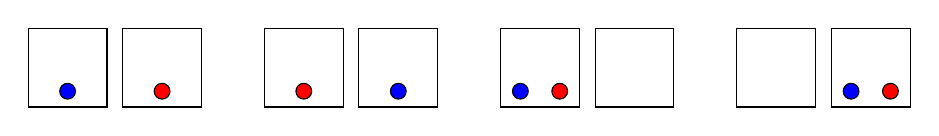
\begin{tikzpicture}
\draw (0,0) rectangle (1,1);
\draw (1.2,0) rectangle (2.2,1);
\draw (3,0) rectangle (4,1);
\draw (4.2,0) rectangle (5.2,1);
\draw (6,0) rectangle (7,1);
\draw (7.2,0) rectangle (8.2,1);
\draw (9,0) rectangle (10,1);
\draw (10.2,0) rectangle (11.2,1);

\draw[fill=blue] (0.5,0.2) circle (0.1);
\draw[fill=red] (1.7,0.2) circle (0.1);
\draw[fill=red] (3.5,0.2) circle (0.1);
\draw[fill=blue] (4.7,0.2) circle (0.1);
\draw[fill=blue] (6.25,0.2) circle (0.1);
\draw[fill=red] (6.75,0.2) circle (0.1);
\draw[fill=blue] (10.45,0.2) circle (0.1);
\draw[fill=red] (10.95,0.2) circle (0.1);
\end{tikzpicture}
\end{center}
此时空盒子数的期望为
\[\frac{0+0+1+1}{4} = \frac{1}{2}.\]
一般情况下，某个盒子为空的概率为
\[\Big(\frac{n-1}{n}\Big)^n,\]
因为没有任何球被放入其中。因此，利用期望的线性性，空盒子数的期望为
\[n \cdot \Big(\frac{n-1}{n}\Big)^n.\]

\subsubsection{概率分布}

\index{distribution}

随机变量 $X$ 的\key{概率分布}给出 $X$ 每个可能取值的概率，由各个 $P(X=x)$ 组成。例如，掷两枚骰子时，点数和的分布为：
\begin{center}
\small {
\begin{tabular}{r|rrrrrrrrrrrrr}
$x$ & 2 & 3 & 4 & 5 & 6 & 7 & 8 & 9 & 10 & 11 & 12 \\
$P(X=x)$ & $1/36$ & $2/36$ & $3/36$ & $4/36$ & $5/36$ & $6/36$ & $5/36$ & $4/36$ & $3/36$ & $2/36$ & $1/36$ \\
\end{tabular}
}
\end{center}

\index{uniform distribution}
在\key{均匀分布}中，随机变量 $X$ 有 $n$ 个可能取值 $a,a+1,\ldots,b$，每个值的概率均为 $1/n$。例如，掷骰子时，$a=1$、$b=6$，每个 $x$ 都有 $P(X=x)=1/6$。

均匀分布中 $X$ 的期望为
\[E[X] = \frac{a+b}{2}.\]

\index{binomial distribution}
在\key{二项分布}中，进行 $n$ 次试验，每次成功的概率为 $p$。随机变量 $X$ 表示成功次数，取值为 $x$ 的概率为
\[P(X=x)=p^x (1-p)^{n-x} {n \choose x},\]
其中 $p^x$、$(1-p)^{n-x}$ 分别对应成功和失败的试验，${n \choose x}$ 表示选择这些成功试验位置的方法数。

例如，掷骰子十次恰好出现三次 6 的概率为 $(1/6)^3 (5/6)^7 {10 \choose 3}$。

二项分布中 $X$ 的期望为
\[E[X] = pn.\]

\index{geometric distribution}
在\key{几何分布}中，每次试验成功的概率为 $p$，并持续试验直到第一次成功。随机变量 $X$ 表示所需试验次数，取值为 $x$ 的概率为
\[P(X=x)=(1-p)^{x-1} p,\]
其中 $(1-p)^{x-1}$ 对应前 $x-1$ 次失败，$p$ 对应第 $x$ 次首次成功。

例如，持续掷骰子直到出现 6，恰好掷 4 次的概率为 $(5/6)^3 1/6$。

几何分布中 $X$ 的期望为
\[E[X]=\frac{1}{p}.\]

\section{Markov 链}

\index{Markov chain}

\key{Markov 链}
% \footnote{A. A. Markov (1856--1922)
% was a Russian mathematician.}
是由状态及状态间转移组成的随机过程。对于每个状态，都已知转移到其他状态的概率。Markov 链可以表示为一张图，其中结点是状态，边是转移。

例如，考虑一栋有 $n$ 层的楼，初始位于 1 楼。每一步随机向上或向下走一层，但在 1 楼时必定向上，在 $n$ 楼时必定向下。问经过 $k$ 步后位于 $m$ 楼的概率。

本题中，每一层楼对应 Markov 链的一个状态。当 $n=5$ 时，图如下：

\begin{center}
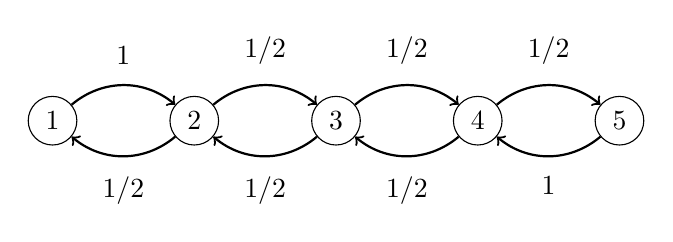
\begin{tikzpicture}[scale=0.9]
\node[draw, circle] (1) at (0,0) {$1$};
\node[draw, circle] (2) at (2,0) {$2$};
\node[draw, circle] (3) at (4,0) {$3$};
\node[draw, circle] (4) at (6,0) {$4$};
\node[draw, circle] (5) at (8,0) {$5$};

\path[draw,thick,->] (1) edge [bend left=40] node[font=\small,label=$1$] {} (2);
\path[draw,thick,->] (2) edge [bend left=40] node[font=\small,label=$1/2$] {} (3);
\path[draw,thick,->] (3) edge [bend left=40] node[font=\small,label=$1/2$] {} (4);
\path[draw,thick,->] (4) edge [bend left=40] node[font=\small,label=$1/2$] {} (5);

\path[draw,thick,->] (5) edge [bend left=40] node[font=\small,label=below:$1$] {} (4);
\path[draw,thick,->] (4) edge [bend left=40] node[font=\small,label=below:$1/2$] {} (3);
\path[draw,thick,->] (3) edge [bend left=40] node[font=\small,label=below:$1/2$] {} (2);
\path[draw,thick,->] (2) edge [bend left=40] node[font=\small,label=below:$1/2$] {} (1);

%\path[draw,thick,->] (1) edge [bend left=40] node[font=\small,label=below:$1$] {} (2);
\end{tikzpicture}
\end{center}

Markov 链的概率分布是向量 $[p_1,p_2,\ldots,p_n]$，其中 $p_k$ 表示当前状态为 $k$ 的概率。始终有 $p_1+p_2+\cdots+p_n=1$。

在上述情形中，初始分布为 $[1,0,0,0,0]$，因为总是从 1 楼开始。下一步的分布为 $[0,1,0,0,0]$，因为从 1 楼只能走到 2 楼。再下一步可以向上或向下走一层，所以分布为 $[1/2,0,1/2,0,0]$，依此类推。

模拟 Markov 链游走的一种高效方法是动态规划：维护概率分布，每一步枚举所有可能转移。利用该方法，可以在 $O(n^2m)$ 时间内模拟 $m$ 步游走。

Markov 链的转移也可以表示为更新概率分布的矩阵。在上述情形中，矩阵为

\[ 
 \begin{bmatrix}
  0 & 1/2 & 0 & 0 & 0 \\
  1 & 0 & 1/2 & 0 & 0 \\
  0 & 1/2 & 0 & 1/2 & 0 \\
  0 & 0 & 1/2 & 0 & 1 \\
  0 & 0 & 0 & 1/2 & 0 \\
 \end{bmatrix}.
\]

用该矩阵乘以概率分布，就得到移动一步后的新分布。例如，可以按下式从分布 $[1,0,0,0,0]$ 转移到 $[0,1,0,0,0]$：

\[ 
 \begin{bmatrix}
  0 & 1/2 & 0 & 0 & 0 \\
  1 & 0 & 1/2 & 0 & 0 \\
  0 & 1/2 & 0 & 1/2 & 0 \\
  0 & 0 & 1/2 & 0 & 1 \\
  0 & 0 & 0 & 1/2 & 0 \\
 \end{bmatrix}
 \begin{bmatrix}
  1 \\
  0 \\
  0 \\
  0 \\
  0 \\
 \end{bmatrix}
=
 \begin{bmatrix}
  0 \\
  1 \\
  0 \\
  0 \\
  0 \\
 \end{bmatrix}.
\]

利用矩阵快速幂，可以在 $O(n^3 \log m)$ 时间内计算 $m$ 步后的分布。

\section{随机化算法}

\index{randomized algorithm}

即使问题本身与概率无关，有时也可以利用随机性求解。\key{随机化算法}就是基于随机性的算法。

\index{Monte Carlo algorithm}

\key{Monte Carlo 算法}是一类有时可能给出错误答案的随机化算法。要让这种算法实用，出错概率必须足够小。

\index{Las Vegas algorithm}

\key{Las Vegas 算法}是一类始终给出正确答案、但运行时间随机变化的随机化算法。目标是让算法以高概率保持高效。

下面介绍三个可以利用随机性解决的示例问题。

\subsubsection{顺序统计量}

\index{order statistic}

数组的第 $k$ 个\key{顺序统计量}，是将数组按升序排序后位于第 $k$ 个位置的元素。先排序可以在 $O(n\log n)$ 时间内求出任意顺序统计量，但仅为寻找一个元素，是否真的需要对整个数组排序？

可以使用随机化算法在不排序整个数组的情况下求顺序统计量。该算法称为\key{快速选择}\footnote{1961 年，C. A. R. Hoare 发表了两种平均效率很高的算法：用于数组排序的\index{quicksort}\key{快速排序} \cite{hoa61a}，以及用于寻找顺序统计量的\index{quickselect}\key{快速选择} \cite{hoa61b}。}，它属于 Las Vegas 算法：通常运行时间为 $O(n)$，最坏情况下为 $O(n^2)$。

算法随机选择数组元素 $x$，把小于 $x$ 的元素移到数组左部，其余元素移到右部。对于 $n$ 个元素，这一步需要 $O(n)$ 时间。假设左部含 $a$ 个元素，右部含 $b$ 个元素。若 $a=k$，则 $x$ 就是第 $k$ 个顺序统计量；若 $a>k$，就在左部递归寻找第 $k$ 个顺序统计量；若 $a<k$，就在右部递归寻找第 $r=k-a$ 个顺序统计量。如此继续，直到找到目标元素。

当每次随机选择 $x$ 时，数组规模在每一步大约减半，因此寻找第 $k$ 个顺序统计量的时间复杂度约为
\[n+n/2+n/4+n/8+\cdots < 2n = O(n).\]

算法最坏情况下仍需 $O(n^2)$ 时间，因为可能每次选到的 $x$ 都是数组中最小或最大的元素之一，从而需要 $O(n)$ 步。不过，这种情况的概率极小，实践中几乎不会发生。

\subsubsection{验证矩阵乘法}

\index{matrix multiplication}

下一个问题是：当 $A$、$B$、$C$ 均为 $n \times n$ 矩阵时，\emph{验证} $AB=C$ 是否成立。当然，可以重新计算乘积 $AB$（基础算法需要 $O(n^3)$ 时间），但验证答案理应有机会比从头计算更容易。

可以使用时间复杂度仅为 $O(n^2)$ 的 Monte Carlo 算法解决该问题\footnote{R. M. Freivalds 于 1977 年发表了该算法 \cite{fre77}，它有时称为\index{Freivalds' algoritm}\key{Freivalds 算法}。}。思想很简单：随机选择一个含 $n$ 个元素的向量 $X$，计算 $ABX$ 和 $CX$。若 $ABX=CX$，就报告 $AB=C$；否则报告 $AB\neq C$。

算法的时间复杂度为 $O(n^2)$，因为 $ABX$ 和 $CX$ 都能在 $O(n^2)$ 时间内计算。把 $ABX$ 写成 $A(BX)$，只需进行两次 $n\times n$ 矩阵与 $n\times1$ 矩阵的乘法，即可高效求出它。

该算法的缺点是：报告 $AB=C$ 时，有很小概率出错。例如，
\[
 \begin{bmatrix}
  6 & 8 \\
  1 & 3 \\
 \end{bmatrix}
\neq
 \begin{bmatrix}
  8 & 7 \\
  3 & 2 \\
 \end{bmatrix},
\]
but
\[
 \begin{bmatrix}
  6 & 8 \\
  1 & 3 \\
 \end{bmatrix}
 \begin{bmatrix}
  3 \\
  6 \\
 \end{bmatrix}
=
 \begin{bmatrix}
  8 & 7 \\
  3 & 2 \\
 \end{bmatrix}
 \begin{bmatrix}
  3 \\
  6 \\
 \end{bmatrix}.
\]
不过在实践中，算法出错的概率很小；在报告 $AB=C$ 之前使用多个随机向量 $X$ 重复验证，可以进一步降低出错概率。

\subsubsection{图着色}

\index{coloring}

给定含 $n$ 个结点和 $m$ 条边的图，任务是用两种颜色给结点着色，使至少 $m/2$ 条边的两个端点颜色不同。例如，对于图
\begin{center}
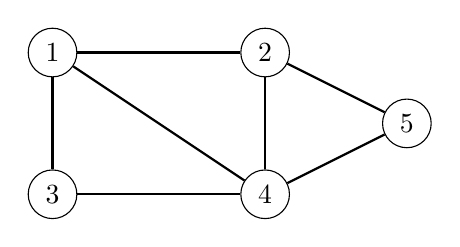
\begin{tikzpicture}[scale=0.9]
\node[draw, circle] (1) at (1,3) {$1$};
\node[draw, circle] (2) at (4,3) {$2$};
\node[draw, circle] (3) at (1,1) {$3$};
\node[draw, circle] (4) at (4,1) {$4$};
\node[draw, circle] (5) at (6,2) {$5$};

\path[draw,thick,-] (1) -- (2);
\path[draw,thick,-] (1) -- (3);
\path[draw,thick,-] (1) -- (4);
\path[draw,thick,-] (3) -- (4);
\path[draw,thick,-] (2) -- (4);
\path[draw,thick,-] (2) -- (5);
\path[draw,thick,-] (4) -- (5);
\end{tikzpicture}
\end{center}
一种合法着色如下：
\begin{center}
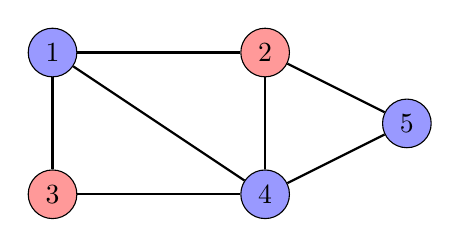
\begin{tikzpicture}[scale=0.9]
\node[draw, circle, fill=blue!40] (1) at (1,3) {$1$};
\node[draw, circle, fill=red!40] (2) at (4,3) {$2$};
\node[draw, circle, fill=red!40] (3) at (1,1) {$3$};
\node[draw, circle, fill=blue!40] (4) at (4,1) {$4$};
\node[draw, circle, fill=blue!40] (5) at (6,2) {$5$};

\path[draw,thick,-] (1) -- (2);
\path[draw,thick,-] (1) -- (3);
\path[draw,thick,-] (1) -- (4);
\path[draw,thick,-] (3) -- (4);
\path[draw,thick,-] (2) -- (4);
\path[draw,thick,-] (2) -- (5);
\path[draw,thick,-] (4) -- (5);
\end{tikzpicture}
\end{center}
上图有 7 条边，其中 5 条边的两个端点颜色不同，因此该着色合法。

可以使用 Las Vegas 算法解决该问题：不断随机生成着色，直到找到合法着色。在随机着色中，每个结点独立选择颜色，两种颜色的概率均为 $1/2$。

在随机着色中，一条边的两个端点颜色不同的概率为 $1/2$。因此，端点颜色不同的边数期望为 $m/2$。由于随机着色在期望意义下就是合法的，实践中很快就能找到一个合法着色。
